%% LaTeX-Beamer template for KIT design
%% by Erik Burger, Christian Hammer
%% title picture by Klaus Krogmann
%%
%% version 2.1
%%
%% mostly compatible to KIT corporate design v2.0
%% http://intranet.kit.edu/gestaltungsrichtlinien.php
%%
%% Problems, bugs and comments to
%% burger@kit.edu

\documentclass[18pt]{beamer}

%% SLIDE FORMAT

% use 'beamerthemekit' for standard 4:3 ratio
% for widescreen slides (16:9), use 'beamerthemekitwide'

\usepackage{templates/beamerthemekit}
% \usepackage{templates/beamerthemekitwide}

%% TITLE PICTURE

% if a custom picture is to be used on the title page, copy it into the 'logos'
% directory, in the line below, replace 'mypicture' with the 
% filename (without extension) and uncomment the following line
% (picture proportions: 63 : 20 for standard, 169 : 40 for wide
% *.eps format if you use latex+dvips+ps2pdf, 
% *.jpg/*.png/*.pdf if you use pdflatex)

%\titleimage{mypicture}

%% TITLE LOGO

% for a custom logo on the front page, copy your file into the 'logos'
% directory, insert the filename in the line below and uncomment it

%\titlelogo{mylogo}

% (*.eps format if you use latex+dvips+ps2pdf,
% *.jpg/*.png/*.pdf if you use pdflatex)

%% TikZ INTEGRATION

% use these packages for PCM symbols and UML classes
% \usepackage{templates/tikzkit}
% \usepackage{templates/tikzuml}

% the presentation starts here
\usepackage{graphicx}
\usepackage{listings}
\usepackage{color}
\usepackage{textcomp}
\definecolor{listinggray}{gray}{0.9}
\definecolor{lbcolor}{rgb}{0.9,0.9,0.9}
\lstset{
	language=Java,
	backgroundcolor=\color{lbcolor},
	tabsize=4,
	rulecolor=,
        basicstyle=\footnotesize,
        aboveskip=5pt,
        upquote=true,
        columns=fixed,
        showstringspaces=false,
        extendedchars=true,
        breaklines=true,
        frame=single,
        showtabs=false,
        showspaces=false,
        showstringspaces=false,
        identifierstyle=\ttfamily,
        keywordstyle=\color[rgb]{0,0,1},
        commentstyle=\color[rgb]{0.133,0.545,0.133},
        stringstyle=\color[rgb]{0.627,0.126,0.941},
}
\usepackage[utf8]{inputenc}

\title[Prog Tut Nr. 5]{Tutorium Programmieren}
\subtitle{Tut Nr.5: Arrays & Javadoc}
\author{Michael Friedrich}
\date{26. / 28.11.2013}

\institute{Institut f\"ur theoretische Informatik}
% Bibliography

\usepackage[citestyle=authoryear,bibstyle=numeric,hyperref,backend=biber]{biblatex}
\addbibresource{templates/example.bib}
\bibhang1em

\begin{document}

% change the following line to "ngerman" for German style date and logos
\selectlanguage{ngerman}

%title page
\begin{frame}
	\titlepage
\end{frame}

%table of contents
\begin{frame}{Outline/Gliederung}
	\tableofcontents
\end{frame}

\section{Allgemeine Anmerkungen}
\begin{frame}[fragile]{WICHTIG}
\begin{itemize}
\item jedes Übungsblatt hat seine eigene Checkstyle XML
\item nur \textbf{grüne} final solutions haben Chance auf \textbf{volle Punktzahl}
\item die Abgaben \textbf{MÜSSEN} gewissen Kriterien genügen, um überhaupt gewertet zu werden \newline
$\Rightarrow$ \textbf{mindestens gelb} \newline
Vergleich: Leserlichkeit bei handschriftlichen Abgaben 
\item Ich war mit der ersten Abgabe zufrieden, daher keine weitere allg. Kommentare
\end{itemize}
\end{frame}


\section{Javadoc}
\begin{frame}[fragile]{Javadoc}
\center{alter Foliensatz}
\end{frame}

\section{Arrays}
\subsection{Deklaration}
\begin{frame}[fragile]{Deklarieren von Arrays}
\begin{itemize}
\item Datenstruktur für eine Sammlung an Daten
\pause
\begin{itemize}
\item Über Indizes einzelne Elemente direkt erreichbar
\pause
\end{itemize}
\end{itemize}
\begin{exampleblock}{Beispiele}
	\begin{lstlisting}
				int[] array;
				
				int[] array = {1,2,3};
				
				int[] array = new int[4];
				
	\end{lstlisting}
\end{exampleblock}
\pause
\begin{itemize}
\item Indizes beginnen immer bei \textbf{ 0} !
\pause
\item Arraygröße abfragen über \lstinline{array.length}
\end{itemize}
\end{frame}

\subsection{Besonderheiten}
\begin{frame}[fragile]{Besonderheiten}
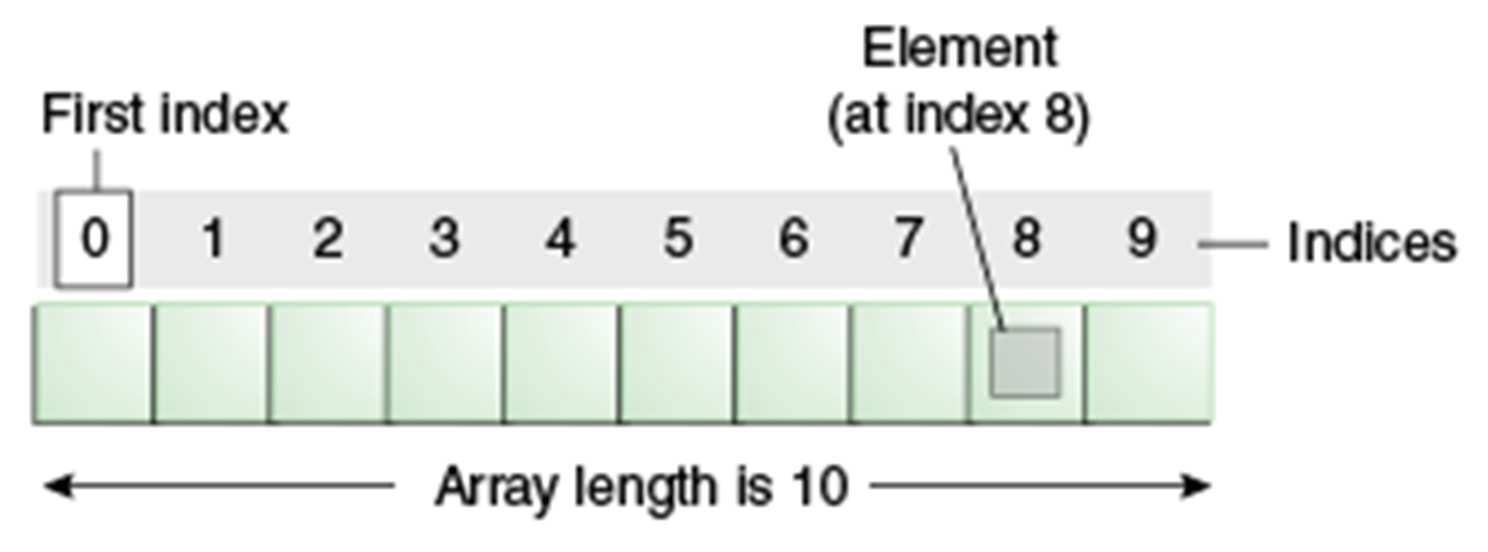
\includegraphics[width=\textwidth]{array.png}
\begin{itemize}
	\item \textbf{Überschreiten} der Grenzen eines Arrays führt zu Exception und damit \textbf{Absturz} eures Programms!
\end{itemize}
\end{frame}

\section{Tutoriumsaufgabe}
\begin{frame}[fragile]{Tutoriumsaufgabe}
\textbf{Arrays - A}
\begin{itemize}

\item \small Schreiben Sie eine Methode \newline
\lstinline{public static int arraySum(int[] array)}, \newline
die die Summe der Zahlen des übergebenen Arrays als Rückgabewert hat.
Schreiben Sie in einer Klasse namens Loops die Methoden

\item Schreiben Sie eine Methode \newline
\lstinline{public static double average(int[] array)}, \newline
die den durchschnittlichen Wert der Zahlen des übergebenen Arrays als Rückgabewert hat.

\item Schreiben Sie eine Methode \newline
\lstinline{public static double[] sum(double[] vectorA, double[] vectorB)}, \newline
die eine Vektoraddition auf den beiden übergebenen Vektoren durchführt und das Ergebnis als
Rückgabewert hat. Achten Sie darauf, dass die beiden Vektoren hierzu dieselbe Länge haben
müssen und dass Sie beim Berechnen der Summe weder vectorA noch vectorB verändern.
\end{itemize}
\end{frame}

\begin{frame}[fragile]{Tutoriumsaufgabe}
\textbf{Arrays - B}
\begin{itemize}

\item \small Schreiben Sie eine Methode \newline
\lstinline{public static double[] scalarMult(double[] vectorA, double scalar)}, \newline
die den Vektor vectorA mit dem Skalar scalar multipliziert und das Ergebnis als Rückgabewert
hat. Achten Sie auch hier darauf, dass vectorA unverändert bleibt.

\item Schreiben Sie eine Methode \newline
\lstinline{public static double[][] sum(double[][] matrixA, double[][] matrixB)}, \newline
die die Matrizen matrixA und matrixB addiert und das Ergebnis als Rückgabewert hat.
Beachten Sie, dass hierzu die Dimensionen der Matrizen gleich sein müssen und dass auch hier
weder matrixA und matrixB verändert werden sollen.
\end{itemize}
\end{frame}

\subsection{Lösung}
\begin{frame}[fragile]{Lösung}
\begin{lstlisting}
static double[] sum(double[] vectorA, double[] vectorB) {
	
	if (vectorA.length != vectorB.length) {
		System.out.println( "Vektoren nicht gleich lang" );
		return null;
	}
	double[] vectorRes = new double[vectorA.length];
	
	for (int i = 0; i < vectorA.length; i++) {
		vectorRes[i] = vectorA[i] + vectorB[i];
	}
	return vectorRes;
}

\end{lstlisting}
\end{frame}

\begin{frame}[fragile]{Lösung}
\begin{lstlisting}[breaklines=false,basicstyle=\tiny]
public static double[][] sum(double[][] matrixA, double[][] matrixB) {
	   double[][] matrixRes;
	
	   //Hinweis: Interne Darstellung mehrdimensionale Arrays: "Ein Array von Arrays"
	   if (matrixA.length != matrixB.length && matrixA[1].length != matrixB.length[2]){
		   	 System.out.println( "Matrizen mit verschiedenen Dimensionen" );
			   return null;
	}
	
	 for (int i = 0; i < a.length; i++) {
		   for (int j = 0; j < a.length; j++) {
			     matrixRes[i][j] = matrixA[i][j] + matrixB[i][j];
		   }
	}
	 return matrixRes;
}
\end{lstlisting}
\end{frame}


\appendix
\beginbackup

%\begin{frame}[allowframebreaks]{References}
%	\printbibliography
%\end{frame}

\backupend

\end{document}
